% -*- TeX -*-

\documentclass{beamer}
\usepackage{amsmath}

\title{PyLith Modeling Tutorial}
\subtitle{Meshing Strategies}
\author{Charles Williams \\
  Brad Aagaard \\
  Matthew Knepley}
\institute{
\includegraphics[scale=0.4]{../../logos/cig_blackfg}}
\date{June 19, 2016}


% ---------------------------------------------------- CUSTOMIZATION
\newcommand{\thispdfpagelabel}[1]{}
\newcommand{\important}[1]{{\color{red}#1}}
\usetheme{CIG}

% --------------------------------------------------------- DOCUMENT
\begin{document}

% ------------------------------------------------------------ SLIDE
\maketitle

% ========================================================== SECTION
\section{Meshing}
\subsection{General steps}

% ------------------------------------------------------------- LOGO
\logo{
\includegraphics[height=4.5ex]{../../logos/cig_blackfg}}

% ------------------------------------------------------------ SLIDE
\begin{frame}
  \frametitle{Meshing Complex Geometry}
  \summary{Steps in creating a mesh}
  
  \begin{itemize}
  \item Determine geometric features needed
    \begin{itemize}
    \item Fault geometry
    \item Topography
    \item Sharp structural boundaries
    \item Magma sources with complex geometry
    \end{itemize}
  \item Create spline curve (2D) or NURBS surface (3D) in CUBIT/Trelis
  \item If using surface in several models export it for future use
  \item Use surfaces within CUBIT/Trelis to webcut volumes
  \item Choose discretization according to type of problem
  \end{itemize}

\end{frame}

% ========================================================== SECTION
\subsection{Meshing examples}

% ------------------------------------------------------------ SLIDE
\begin{frame}
  \frametitle{Example problems}
  \summary{3-D meshing of nonplanar geometry and variable discretization}
  
  \begin{itemize}
  \item Three-dimensional subduction zone example using NURBS surfaces\\
    \important{{\tt examples/meshing/surface\_nurbs/subduction}}
    \begin{itemize}
    \item Subduction interface geometry
    \item Splay fault geometry
    \item Topography/bathymetry
    \end{itemize}
  \item How to use CUBIT's sizing function to vary discretization size\\
    \important{{\tt examples/meshing/cubit\_cellsize}}
  \end{itemize}
  \vfill
  \important{These examples have been verified to work with CUBIT 15.1
    and Trelis 16.0.2.}


\end{frame}


% ========================================================== SECTION
\subsection{3-D Subduction}

% ------------------------------------------------------------ SLIDE
\begin{frame}
  \frametitle{3-D Subduction Zone}
  \summary{Mesh with subduction thrust, splay fault, and topo/bathymetry}
 
  \vfill
  \begin{center}
    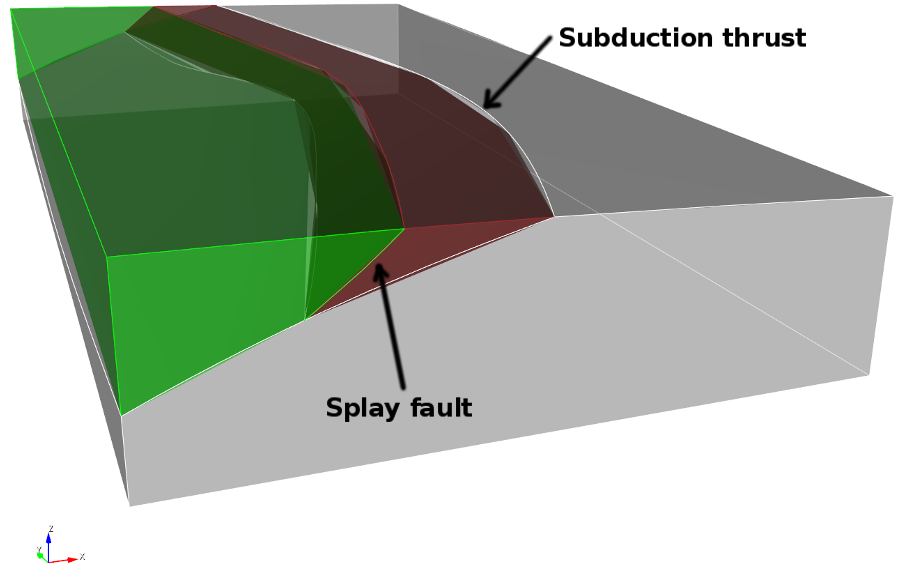
\includegraphics[width=4.5in]{figs/subduction3d_geometry}
  \end{center}
  \vfill

\end{frame}


% ========================================================== SECTION
\subsection{CUBIT Sizing Function}

% ------------------------------------------------------------ SLIDE
\begin{frame}
  \frametitle{Using user-defined fields to control mesh size}
  \summary{Example 1: Use a spatial database to control cell size}
 
  Cell size field\\
  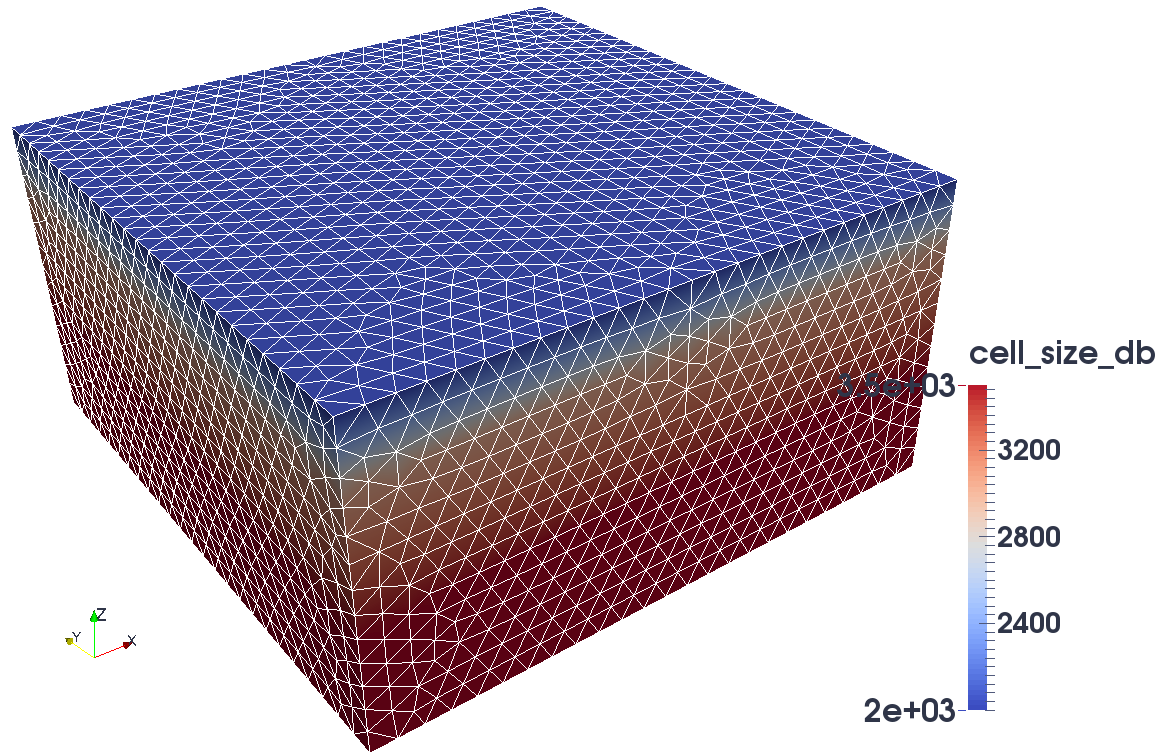
\includegraphics[height=7.1cm]{figs/cellsize_spatialdb}
 
\end{frame}


% ------------------------------------------------------------ SLIDE
\begin{frame}
  \frametitle{Using user-defined fields to control mesh size}
  \summary{Example 1: Use a spatial database to control cell size}
 
  Resulting mesh\\
  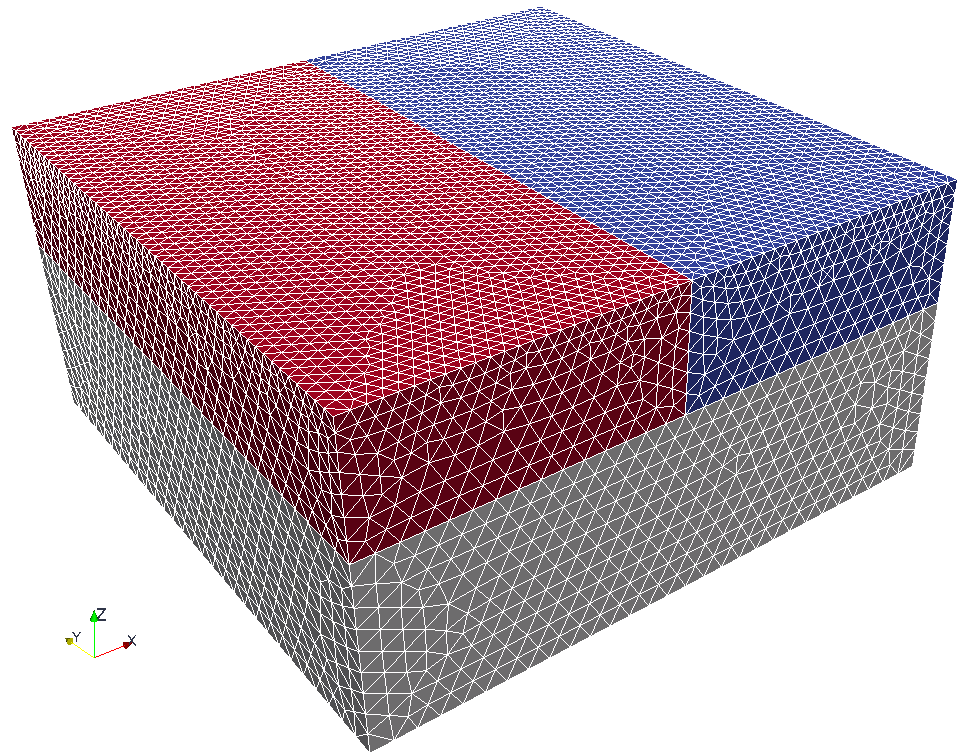
\includegraphics[height=7.1cm]{figs/cellsize_spatialdb_mesh}
 
\end{frame}


% ------------------------------------------------------------ SLIDE
\begin{frame}
  \frametitle{Using user-defined fields to control mesh size}
  \summary{Example 2: Use an analytical function to control cell size}
 
  Cell size field\\
  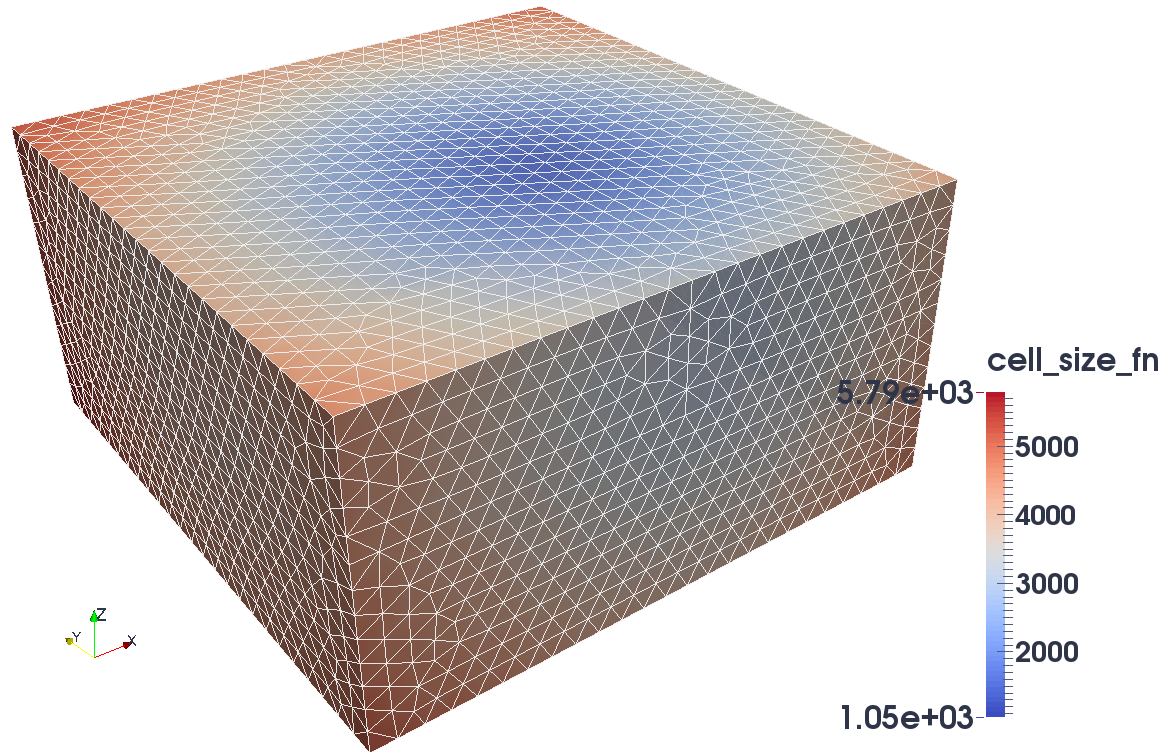
\includegraphics[height=7.1cm]{figs/cellsize_analyticfn}
 
\end{frame}
 

% ------------------------------------------------------------ SLIDE
\begin{frame}
  \frametitle{Using user-defined fields to control mesh size}
  \summary{Example 2: Use an analytical function to control cell size}
 
  Resulting mesh\\
  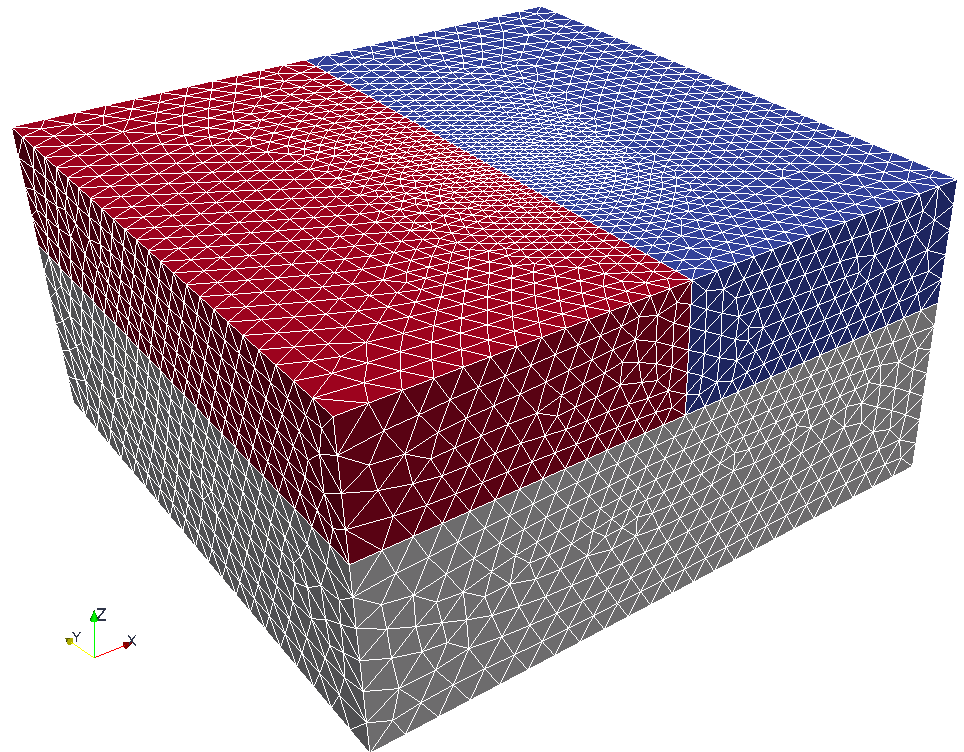
\includegraphics[height=7.1cm]{figs/cellsize_analyticfn_mesh}
 
\end{frame}
 

% ======================================================================
\end{document}


% End of file
